\documentclass[a4paper]{article}

%% Language and font encodings
\usepackage[english]{babel}
\usepackage[utf8x]{inputenc}
\usepackage[T1]{fontenc}

%% Sets page size and margins
\usepackage[a4paper,top=3cm,bottom=2cm,left=3cm,right=3cm,marginparwidth=1.75cm]{geometry}

%% Useful packages
\usepackage{amsmath}
\usepackage{graphicx}
\usepackage[colorinlistoftodos]{todonotes}
\usepackage[colorlinks=true, allcolors=blue]{hyperref}

\usepackage{caption}
\usepackage{subcaption}

\graphicspath{{res/}}

\title{Signal Analysis with the Fourier Transform, Correlation Theorem, and Sideband Mixers}
\author{Lukas Finkbeiner}

\begin{document}
\maketitle

\begin{abstract}

We investigate aliasing and confirm the Nyquist criterion by signals at various ratios of the sampling frequency and find that deterioration in the sample's facsimile is independent of the ability to reconstruct the signal with a power spectrum. Through frequency resolution and power leakage, we demonstrate the data-analysis consequences of the discrete bounded Fourier transform as compared to the ideal. We apply similar methods and analyses to synthesized noise and comment on the implications for averaging as a noise-compensation mechanism. We verify the trigonometry desired of double sideband mixers while acknowledging the shortcomings of nonlinear diodes with regards to intermodulation.

\end{abstract}

% No need to re-derive anything!!

\section{Introduction and Background}

Let $V(t)$ be voltage as a function of time and $V(\nu)$ the corresponding voltage as a function of frequency $\nu$.

\

$V(\nu) = \int_{-T / 2}^{T / 2} V(t) \exp(2 \pi i \nu t) dt$ and $V(t) = \frac{1}{\nu_s} \int_{- \nu_s / 2}^{\nu_s / 2} \tilde{V}(\nu) \exp(-2 \pi i \nu t) d \nu$

\

Where T is the length of the time sample, and $\nu_s$ is the sampling frequency used.


% ?? I need to talk about Parseval's Theorem


The sine function is odd: $\sin(-\omega t) = -sin(\omega t)$. The cosine function is even: $\cos(-\omega t) = \cos (\omega t)$.

We can generalize under Euler's identity: $A\exp(i \omega t) = A \cos(\omega t) + i \cdot A \sin(\omega t)$ such that $A\exp(-i \omega t) = A \cos(-\omega t) + i \cdot A \sin(-\omega t) = A \cos(\omega t) - i \cdot A \sin(\omega t)$.

This allows us to accept negative and imaginary frequencies, which are nominally unphysical, as consequences of phase shift. For example, a signal and its flipped counterpart could be said to have opposite frequencies.

In the laboratory, we cannot use the ideal of an unbounded Fourier transform (as in, the limits of integration are $\pm \infty$), because we have to start sampling at some point and stop sampling at another. Furthermore, we cannot use the continuous Fourier transform because we collect data as snapshots, as individual poins. Consequently, we cannot perform an integral but instead a sum. 

Nyquist's criterion sates that the sampling frequency must exceed the maximum signal frequency by a factor of two. If it does not, aliasing causes the signal to be irretrievable through the discrete and bounded Fourier transform; to reproduce any periodic shape, one needs over 2 points per period in order to guarantee that the shape is not mistaken for another of a different period.

We define the convolution and correlation of two functions $f(t)$ and $g(t)$, respectively, as:

\

$[f * g](\tau) = \int_{-T / 2}^{T / 2} f(t) g(\tau - t) dt$ \quad and \quad $[f \star g](\tau) = \int_{-T / 2}^{T / 2} f(t) g(\tau + t) dt$

\section{Methods}

%\quad \quad This is the equipment I used. These are the libraries and functions I used. This is how I used them ($vague$ hint at your code). Uncertainty? Technical errors?

\quad \quad To begin our investigation of the Nyquist criterion, we decided on a sampling frequency $\nu_s = 6.25$ MHz at which the pico sampler (a PicoScope 2206A) remained for the duration of the data collection for all signals. We then used the N9310A RF Signal Generator to output signals at frequency $\nu_0$: fractions of the sampling frequency. For example, one of our input signals was $\nu_0 = .4 \nu_s = 2.5$ MHz. For all signals, we performed visual inspections of the pico sampler's input by using a T-joint and connecting the output to an oscilloscope (a Rigol DS1052E). We used the ugradio module to perform data collection (ugradio.pico.capture\_data) and, later on, to perform Fourier and inverse Fourier transforms (ugradio.dft.dft and ugradio.dft.idft).

To consider the frequency resolution for two signals of similar frequency, we employed a second signal generator. The 83712B has a lower limit of 10 MHz output frequency. Consequently, we set our original signal generator to small increments above that frequency and needed to increase the sampling frequency to $\nu_s = 31.25$ MHz.

To investigate the impact of noise on the Fourier transform, we switched the pico sampler's input to an NOD 5250 noise generator (6 MHz bandpass) at zero attenuation. We collected 32 blocks of 16000 samples from the PicoScope, this time using the sampling frequency $\nu_s = 62.5$ MHz.

We explored mixers and sideband theory with a Mini-Circuits ZAD-1. We the 83712B as the local oscillator and the N9310A as the RF input. We sent the output to the oscilloscope and PicoScope, this time using a $50 \Omega$ terminator to eliminate bounce-back interference. The ZAD-1 works best for signals above 10 MHz, so we set the local oscillator to $\nu_{LO} = 11$ MHz and collected two sets of data: one for which $\nu_{RF} = 11.55$ MHz and one for which $\nu_{RF}=10.45$ MHz (thus, $\Delta \nu = .05 \nu_{LO} = .55$ MHz. 

The mixed signals were somewhat weak, so we used 1.5 dBm amplitudes on both signal generators. We again used a sampling frequency of $\nu_s = 62.5$ MHz, motivated by the following identities:

$\sin(\nu_{LO}) \sin(\nu_{LO} + \Delta \nu) = \frac{1}{2} (\cos \Delta \nu - \cos (2\nu_{LO} + \Delta \nu))$ by evenness of the cosine function

$\sin(\nu_{LO}) \sin(\nu_{LO} - \Delta \nu) = \frac{1}{2} (\cos \Delta \nu - \cos (2\nu_{LO} - \Delta \nu))$

Now, if we expect to see two signals, $2\nu_{LO} + \Delta \nu = 23.1$ 23.1 is the highest frequency that we would expect. Our PicoScope offers sampling rates by dividing the base $62.5$ MHz. 31.25 MHz would have failed the Nyquist criterion, so we used the maximum sampling rate instead. 

Finally, we constructed a single-sideband mixer by using two mixers. Both mixers used both the local oscillator and radio frequency signals, but one of the mixers' RF input was phase shifted by approximately $\pi / 2$ by linking smaller cables together until we roughly satisfied the $\lambda / 4$ criterion.

%\textcolor{red}{I don't remember the model of the other mixer} 

\section{Results}

\subsection{Nyquist Sampling}

% subsection{5.2}

\quad \quad We took the default 16000 samples for each of our first signal samples. However, for the data analysis, we will be excluding the first 100 samples due to a peculiarity of the pico sampler which distorted these (see figure \ref{fig:pico_start}).

% Perhaps not important to discuss differences in peak to peak voltages across trials

\begin{figure}
\centering
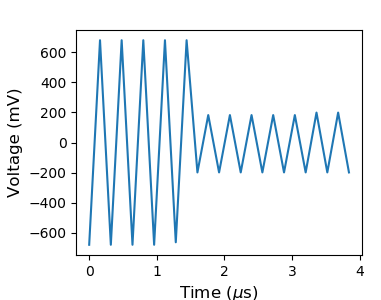
\includegraphics[width=0.3\textwidth]{5-2/pico_bad}
\caption{The oscilloscope displayed a constant signal throughout the period of data-taking. The data sampled from the pico sampler, however, reconstructs a signal with large aberrations in the first few microseconds.}
\label{fig:pico_start}
\end{figure}

\begin{figure}
\centering
\begin{minipage}{.5\textwidth}
	\centering
	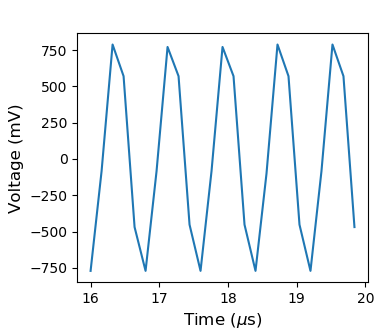
\includegraphics[width=.8\linewidth]{5-2/trial2}
	\caption{$\nu_0 = .2 \nu_s = 1.25$ MHz.}
	\label{fig:Nyq2}
\end{minipage}%
\begin{minipage}{.5\textwidth}
	\centering
	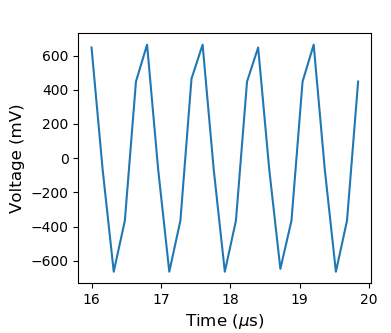
\includegraphics[width=.8\linewidth]{5-2/trial8}
	\caption{$\nu_0 = .8 \nu_s = 5$ MHz.}
	\label{fig:Nyq8}
\end{minipage}
\end{figure}

\begin{figure}
\centering
\begin{minipage}{.5\textwidth}
	\centering
	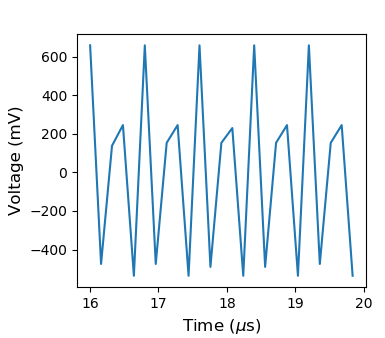
\includegraphics[width=.8\linewidth]{5-2/trial4}
	\caption{$\nu_0 = .4 \nu_s = 2.5$ MHz.}
	\label{fig:Nyq4}
\end{minipage}%
\begin{minipage}{.5\textwidth}
	\centering
	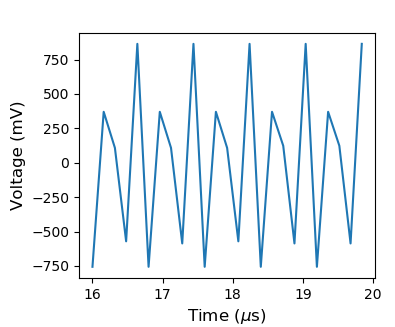
\includegraphics[width=.8\linewidth]{5-2/trial6}
	\caption{$\nu_0 = .6 \nu_s = 3.75$ MHz.}
	\label{fig:Nyq6}
\end{minipage}
\end{figure}
	
We may begin inspection of the samples with a qualitative approach. Figure \ref{fig:Nyq2} shows a signal which repeats about five times in the span of about 4 microseconds. This gives us 1.25 cycles per microsecond, or 1.25 MHz, as expected. Figure \ref{fig:Nyq8} still appoars as a sine wave, but visual inspection is no longer reliable. Again: we see about 5 samples in the span of about 4 microseconds. This would give 1.25 MHz, but because we know that our input signal was in fact $\nu_0 = 5$ MHz, we know that the waveform is aliased.

A more nuanced example comes from frequencies close to $.5 \nu_s$: compare figures \ref{fig:Nyq4} and \ref{fig:NyPw6}. Keeping in mind that only the frequency varied between trials and not the shape of the signal, a visual inspection is now confused: the sample looks like a sine wave in neither case. If take for granted that \ref{fig:Nyq4} is not a perfect sample, we may still visually estimate the frequency by noting 10 pairs of relative extrema (2.5 MHz). 

% ?? Maybe I should put these annotations in the captions (it would be more appropriate there, I think)

% ?? These figures need annotations. You can probably just do the same qualitative thing that you did before.

The power spectra exactly confirm these estimations. Furthermore, there are no obvious aberrations in the power spectra to indicate whether the signal was aliased during sampling. Consider, for example, that figures \ref{fig:NyPw4} and \ref{fig:NyPw6} are identical. An argmax function yielded precisely the same values for the frequency peaks.

The power spectrum for our fifth trial ($\nu_0 = .5 \nu_s = 3.125$ MHz) yielded an argmax with many digits (all other power spectra, even the aliased, returned frequencies to two decimal places). In other words, the calculation becomes more sensitive in a small region around this midpoint. All frequencies above this returned incorrect maxima in the power spectrum, so we have verified the Nyquist criterion. 

%\textcolor{red}{?\? No value and no uncertainty for this trial}

\begin{figure}
\centering
\begin{minipage}{.5\textwidth}
	\centering
	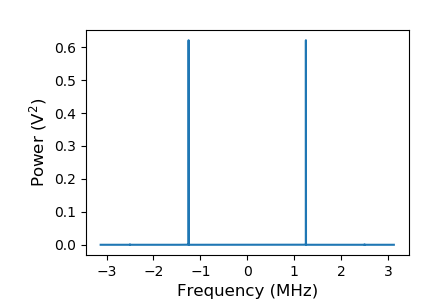
\includegraphics[width=.8\linewidth]{5-2/pow2}
	\caption{$\nu_0 = .2 \nu_s = 1.25$ MHz. Peak amplitudes at $\pm$ 1.25 MHz}
	\label{fig:NyPw2}
\end{minipage}%
\begin{minipage}{.5\textwidth}
	\centering
	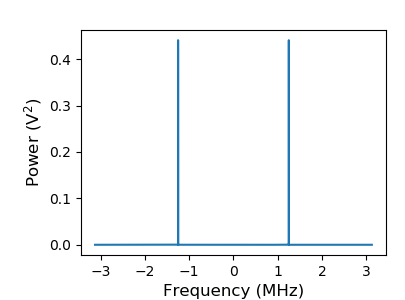
\includegraphics[width=.8\linewidth]{5-2/pow8}
	\caption{$\nu_0 = .8 \nu_s = 5$ MHz. Peak amplitudes at $\pm$ 1.25 MHz}
	\label{fig:NyPw8}
\end{minipage}
\end{figure}

\begin{figure}
\centering
\begin{minipage}{.5\textwidth}
	\centering
	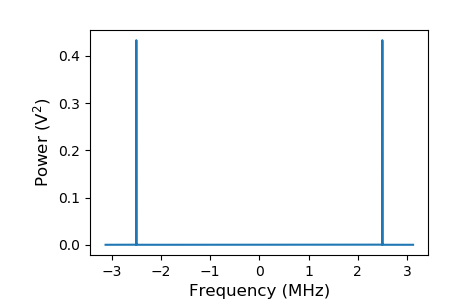
\includegraphics[width=.8\linewidth]{5-2/pow4}
	\caption{$\nu_0 = .4 \nu_s = 2.5$ MHz. Peak amplitudes at $\pm$ 2.5 MHz}
	\label{fig:NyPw4}
\end{minipage}%
\begin{minipage}{.5\textwidth}
	\centering
	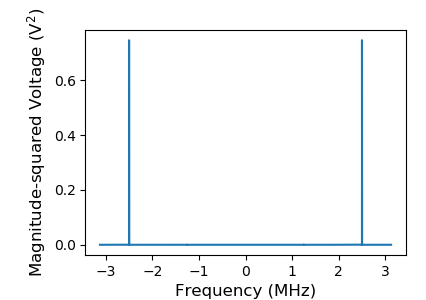
\includegraphics[width=.8\linewidth]{5-2/pow6}
	\caption{$\nu_0 = .6 \nu_s = 3.75$ MHz. Peak amplitudes at $\pm$ 2.5 MHz}
	\label{fig:NyPw6}
\end{minipage}
\end{figure}

% subsection{5.3}

The power spectra show two spikes symmetric about 0. We see them at the positive and negative of (for the non-aliased samples) the input frequency. We can consider the concept of a negative frequency in a broader context by returning to Euler's identity as recalled in the introduction.

Specifically, we calculated the voltage spectra of our samples. Since this is directly the Fourier transform, we now see real and imaginary components which are not visible in the power spectrum due to the magnitude-square operation applied to the outputs.

Differences between voltage spectra of the same signal suggest that variation in imaginary and real components are consequences of phase shifts. Taking multiple blocks of data one after the other (which loosely controls for environmental variation) allows the PicoScope to begin taking data points such that the signals do not overlap.

Power spectra are provided alongside the voltage spectra to demonstrate the power spectrum's destruction of information. The power spectrum does not change (figures \ref{fig:SyPw1}, \ref{fig:SyPw2}, and \ref{fig:SyPw3} are identical) and exhibits complete symmetry always. The voltage spectra, by contrast, are inconsistent. However, excepting noise, which seems to be influencing the patterns at the centers, the spectra are symmetric and antisymmetric in their real and imaginary components, respectively.

% it would be kind of cool to overplot all three waveforms, in different colors...

\begin{figure}
\centering
\begin{minipage}{.5\textwidth}
	\centering
	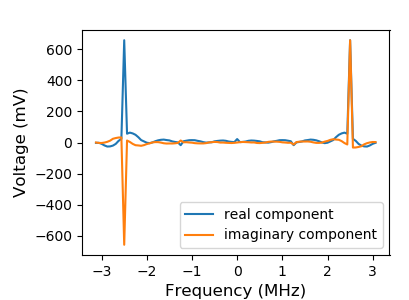
\includegraphics[width=.8\linewidth]{5-3/volt1}
	\caption{Voltage}
	\label{fig:Volt1}
\end{minipage}%
\begin{minipage}{.5\textwidth}
	\centering
	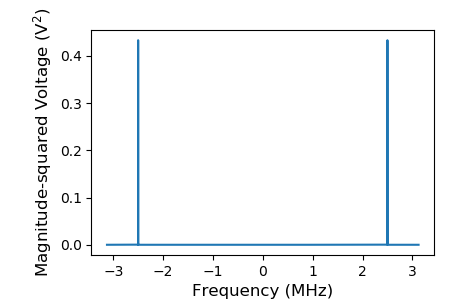
\includegraphics[width=.8\linewidth]{5-3/pow1}
	\caption{Powerish}
	\label{fig:SyPw1}
\end{minipage}
\end{figure}

\begin{figure}
\centering
\begin{minipage}{.5\textwidth}
	\centering
	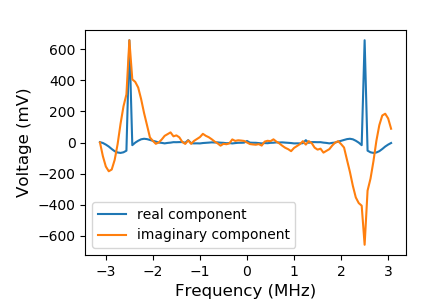
\includegraphics[width=.8\linewidth]{5-3/volt2}
	\caption{Voltage}
	\label{fig:Volt2}
\end{minipage}%
\begin{minipage}{.5\textwidth}
	\centering
	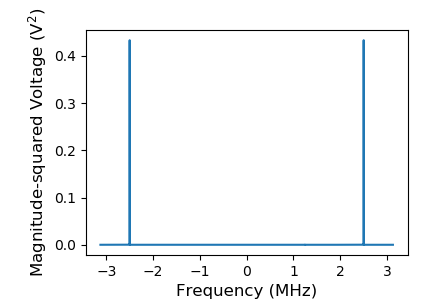
\includegraphics[width=.8\linewidth]{5-3/pow2}
	\caption{Powerish}
	\label{fig:SyPw2}
\end{minipage}
\end{figure}

\begin{figure}
\centering
\begin{minipage}{.5\textwidth}
	\centering
	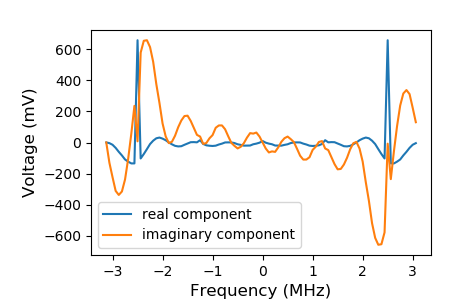
\includegraphics[width=.8\linewidth]{5-3/volt3}
	\caption{Voltage}
	\label{fig:Volt3}
\end{minipage}%
\begin{minipage}{.5\textwidth}
	\centering
	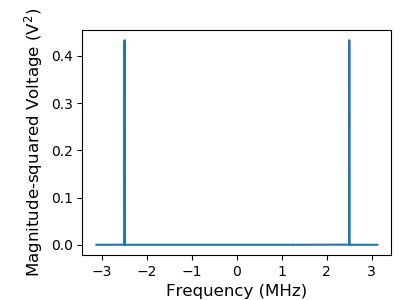
\includegraphics[width=.8\linewidth]{5-3/pow3}
	\caption{Powerishy Squishy}
	\label{fig:SyPw3}
\end{minipage}
\end{figure}

``you need to make sure dft.idft correctly infers the frequencies corresponding to each bins in your power spectrum array''

``When calculating a digital version of the correlation function, you have to worry about end effects.
Suppose you are calculating an ACF for N samples with delays ∆N ranging up to N/2. Then the
number of terms in the sum is always smaller than N because the delays spill over the edge of the
available samples.''

\textcolor{red}{How am I supposed to account for this?}

\begin{figure}
\centering
\begin{minipage}{.5\textwidth}
	\centering
	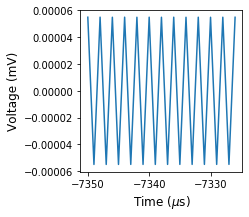
\includegraphics[width=.8\linewidth]{5-3/dft_idft}
	\caption{\textcolor{red}{This is supposed to be the dft/idft version}}
	\label{fig:inverse}
\end{minipage}%
\begin{minipage}{.5\textwidth}
	\centering
	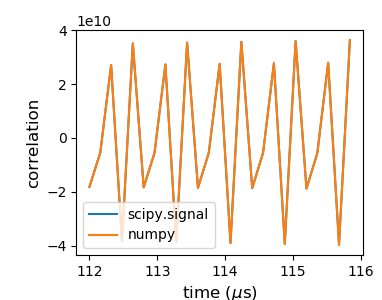
\includegraphics[width=.8\linewidth]{5-3/ACF}
	\caption{Powerish}
	\label{fig:ACF}
\end{minipage}
\end{figure}

Unfortunately, a meaningful discussion of the autocorrelation function (ACF) and its relation to the Fourier transform cannot proceed on experimental results. The convolution and correlation theorems are as follows:

$\widetilde{[f * g]}(\nu) \equiv \int_{-T / 2}^{T / 2}[f * g](\tau) \exp{2 \pi i \tau \nu} d \tau = \tilde{f}(\nu) \cdot \tilde{g}(\nu)$

\

$\widetilde{[f \star g]}(\nu) \equiv \int_{-T / 2}^{T / 2}[f \star g](\tau) \exp{2 \pi i \tau \nu} d \tau = \tilde{f}(\nu) \cdot \tilde{g^*}(\nu)$

If we use the ACF, and say that f and g are the same function, we see that the correlation theorem gives back $\widetilde{[f \star f]}(\nu) = \tilde{f}(\nu) \cdot \tilde{f^*}(\nu) \equiv ||f(\nu)||^2$. However, the right hand side is now our definiton of the power spectra $||V(\nu)||^2$ because we want to perform all such autocorrelations and Fourier transforms on our voltage time series data.

Now, if we take the inverse Fourier transform of both sides, we see that the autocorrelation function $f \star f$ should be the same as the inverse Fourier transform of the power spectrum.

Figure \ref{fig:inverse} shows a slice of the inverse Fourier transform for the $\nu_0 = .4 \nu_s = 2.5$ MHz power spectrum. If the reader will forgive the negative time translation and the lack of normalization, the more alarming issue of crude wave recreation may be observed. Why has the power spectrum, which corresponded to a smooth sine wave, been reduced like so? The data analysis elsewhere in this report has held up well, and this problem persists through multiple trials, so the problem must be in the implementation and understanding of the computer code for this discussion.

Figure \ref{fig:ACF} shows the results of the autocorrelation of that same signal. The results using scipy and numpy are overlaid, but one can hardly tell because there is no discrepancy whatsoever (which suggests that the implementations are fundamentally the same). One might point out that this signal could perhaps simply be a more nuanced version of the same shape as in \ref{fig:inverse}, a much more zoomed out comparison of the two plots will show that the autocorrelation function represents a linear increase from the outer limits to the center: an array of length 31972. The dft/idft, by contrast produces a mostly consistent zig-zag with slight dips on larger-cales, and represents an array of length 16000 (the target length, given our sample size).

% subsection 5.4

\begin{figure}
\centering
\begin{minipage}{.5\textwidth}
	\centering
	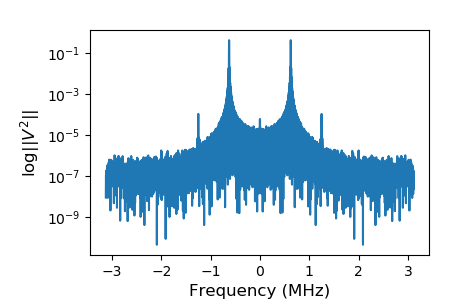
\includegraphics[width=\linewidth]{5-4/t1_eighth}
	\caption{$\nu_0 = .1 \nu_s = .625$ MHz}
	\label{fig:tenth_leakage}
\end{minipage}%
\begin{minipage}{.5\textwidth}
	\centering
	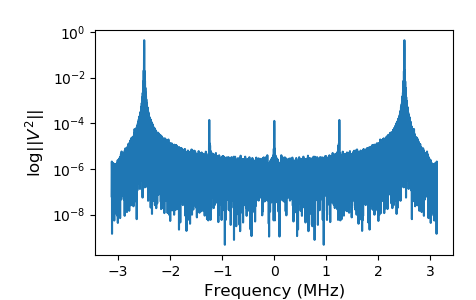
\includegraphics[width=\linewidth]{5-4/t4_eighth}
	\caption{$\nu_0 = .4 \nu_s = 2.5$ MHz}
	\label{fig:4tenths_leakage}
\end{minipage}
\end{figure}

%Recall that spectral leakage is introduced by the finite bounds on our Fourier transforms. Why does that math correspond to these results?

In physical applications, all of our Fourier transforms must be discrete and have finite bounds. Finite bounds introduce spectral leakage, which in fact can be seens regardless of one's changing $\Delta \nu$. However, the effect is particularly pronounced when decreasing $\Delta \nu$. 

Based on our results, we may suggest that spectral leakage becomes an increasingly impactful problem as one approaches the Nyquist criterion. To be sure, there is a variant pattern at the lower end of each leakage pattern, but this seems to stem more from noise than from the leakage pattern in particular. Consider figures \ref{fig:tenth_leakage} and \ref{fig:4tenths_leakage}. The as $\nu_0$ increases in proportion to $nu_s$, we see the erroneous spikes increase in eminence. In fact, in figure \ref{fig:4tenths_leakage}, the leakage spikes overshadow the expected power spikes which we demonstrated earlier. By decreasing the size of the frequency interval, we are computationally introducing additional aliasing into data we have already collected, by treating irregular patterns as single cycles rather than combinations of the same sine wave sampled with different offsets.


% ?? You didn't mention convolutions

% subsection{5.5}

\begin{figure}
\centering
\begin{minipage}{.5\textwidth}
	\centering
	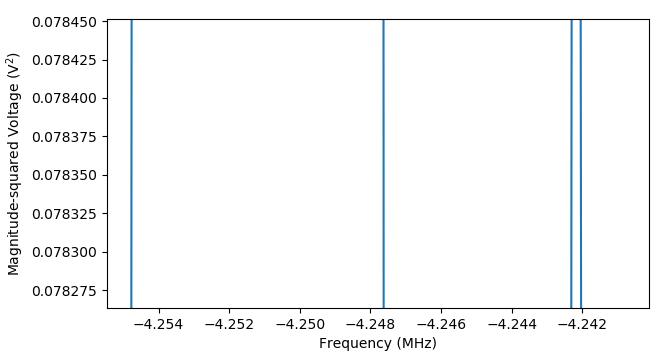
\includegraphics[width=.9\linewidth]{5-5/10k_factor8}
	\caption{Gap of 10kHz between the \hfill \break two frequencies. Here we have decreased \hfill \break $\Delta \nu$ to $v_s / (8N)$.}
	\label{fig:10kf8}
\end{minipage}%
\begin{minipage}{.5\textwidth}
	\centering
	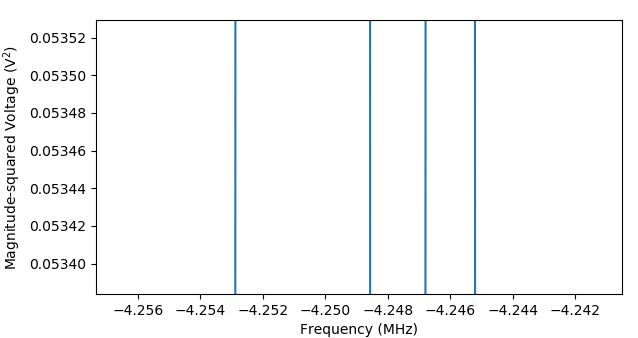
\includegraphics[width=.9\linewidth]{5-5/5k_factor16}
	\caption{Gap of 10kHz between the two frequencies. Here we have decreased $\Delta \nu$ to $v_s / (16N)$.}
	\label{fig:5kf16}
\end{minipage}
\end{figure}

While a decrease in $\Delta \nu$ with respect to $\nu_s$ can introduce unwanted/fictitious signals, it can also allow us to see signals close together, which would otherwise be lumped together.

With one signal generator at 10 MHz, we varied the other with a pseudo-logarithmic pattern: 10.0001, 10.0005, 10.001, 10.005, and 10.01 MHz. In the analysis, we found that our last couple of trials were approaching the end of distinguishability. Figures \ref{fig:10kf8} and \ref{fig:5kf16} represent zoomed in figures which only serve to demonstrate that the signals are separable (consider, for example, the miniscule range of the x-axes).

A factor of two decrease in $\Delta \nu$ allowed us to distinguish between frequencies gaps which were themselves separated by a factor of two. In a discrete Fourier transformation with a difference $\Delta \nu$ instead of a continuous infinitesimal integration parameter $d\nu$, our ability to distinguish two signals of similar frequencies is diminished by aliasing, which will normally be able to pick out a signal between 10 MHz and the other ($\approx$ 10 MHz). By decreasing our $\Delta \nu$ we come closer to approximating a continuous Fourier transform and can separate the two signals.

\subsection{5.6}

\begin{figure}
\centering
\begin{minipage}{.5\textwidth}
	\centering
	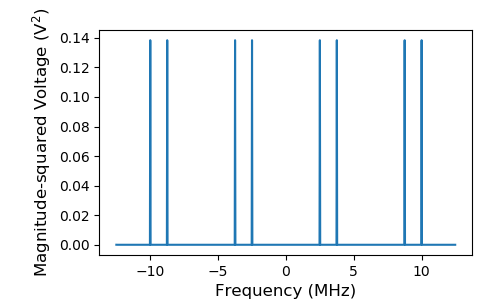
\includegraphics[width=.9\linewidth]{5-6/4window}
	\caption{$\nu_0 = .4 \nu_s = 2.5$ MHz. Fourth window.}
	\label{fig:win4}
\end{minipage}%
\begin{minipage}{.5\textwidth}
	\centering
	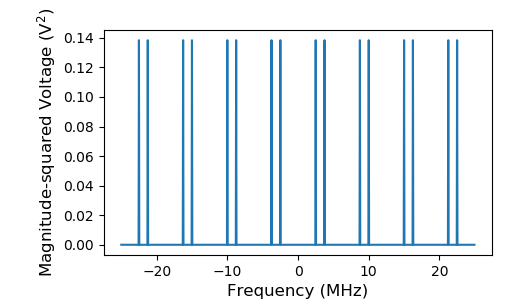
\includegraphics[width=.9\linewidth]{5-6/8window}
	\caption{Same frequency. Eighth window.}
	\label{fig:win8}
\end{minipage}
\end{figure}

\begin{figure}
\centering
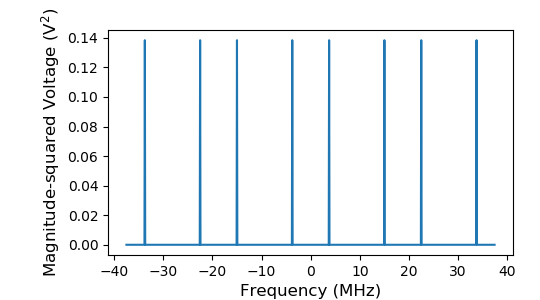
\includegraphics[width=.45\linewidth]{5-6/12window}
\caption{Same frequency. Twelfth window.}
\label{fig:win12}
\end{figure}

As we take the power spectrum out to increasing frequency ranges, we observe repetitions of the original signal which do not strictly increase in frequency, perhaps due to aliasing wrap-around.

Figures \ref{fig:win4}, \ref{fig:win8}, \ref{fig:win12} all represent power spectra for the same data and therefore also for the same input signal frequency. We continue to see pairs of spikes symmetric about the zero frequency. While the number of spike pairs increases dramatically from the fourth (figure \ref{fig:win4}) to the eighth window (\ref{fig:win8}), we see the number drop off steeply by the twelfth window. % What is your point here? I mean, it kind of feels like we're just rambling. Maybe I should cut more closely to the lab manual.

% They can't be harmonics; why else would all the spikes have the same amplitudes. And, for that matter, why do all windows show such low amplitudes? Ah, it is because the input signal (as seen on the oscilloscope) has a much lower amplitude--squaring further affects to that end. ??

\subsection{5.7}

First sample:

Mean = 3.79875 (mV)$^2$

Variance = 412.3663734375 (mV)$^4$

Standard deviation = 20.30680608656861 (mV)$^2$

\begin{figure}
\centering
\begin{minipage}{.5\textwidth}
	\centering
	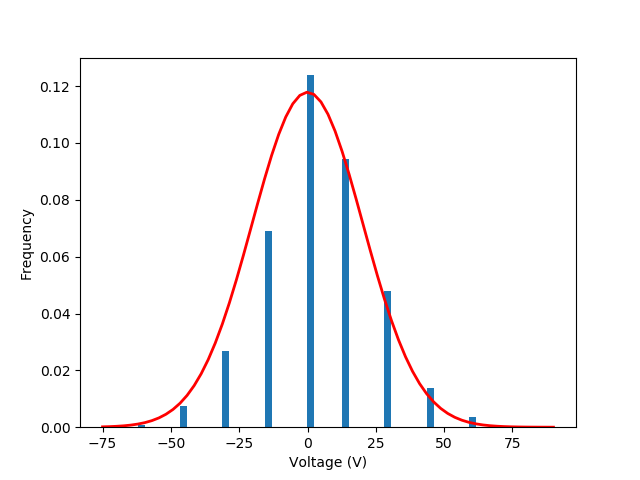
\includegraphics[width=.9\linewidth]{5-7/histo}
	\caption{}
	\label{fig:histogram}
\end{minipage}%
\begin{minipage}{.5\textwidth}
	\centering
	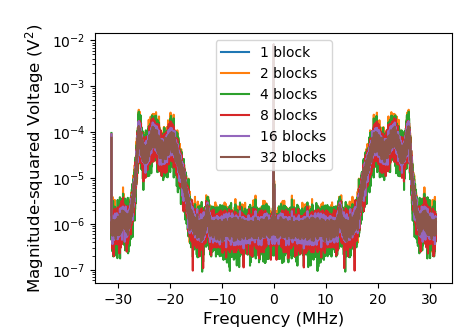
\includegraphics[width=.9\linewidth]{5-7/comparison}
	\caption{}
	\label{fig:avgs_comparison}
\end{minipage}
\end{figure}

\begin{figure}
\centering
\begin{minipage}{.5\textwidth}
	\centering
	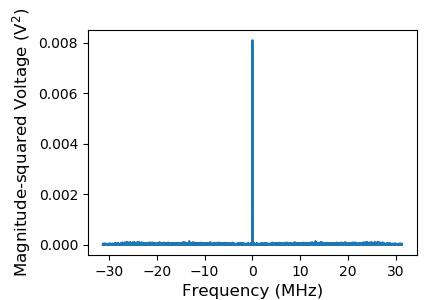
\includegraphics[width=.9\linewidth]{5-7/pow1}
	\caption{}
	\label{fig:pow1}
\end{minipage}%
\begin{minipage}{.5\textwidth}
	\centering
	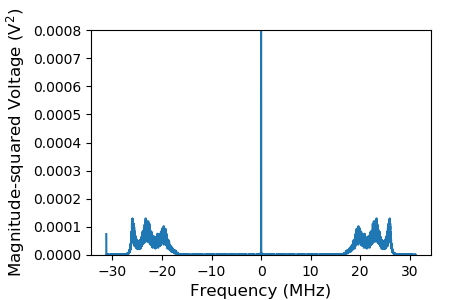
\includegraphics[width=.9\linewidth]{5-7/pow_all}
	\caption{}
	\label{fig:pow_all}
\end{minipage}
\end{figure}

Based on a visual inspection of \ref{fig:avgs_comparison}, the signal to noise ratio power law, as it depends on the number of blocks $N$ used in the sample, is difficult to see. The differences on the logarithmic plot are difficult to see, and it is unclear whether $x$ (as in, signal to noise ratio $\propto N^x$) would be much larger than one tenth. 

Again, the ACF analysis failed. Please refer to the earlier analysis for a discussion of the ACF as well as the correlation and convolution theorems.

\subsection{Mixers}

%section 7.1

Figure \ref{fig:low_display} demonstrates the principle from earlier that a sample can reconstruct a signal (e.g. via Fourier decomposition) without precise visual mimicry. In this case, each cycle of the original signal has produced a visually different sampled cycle. 

\begin{figure}
\centering
\begin{minipage}{.5\textwidth}
	\centering
	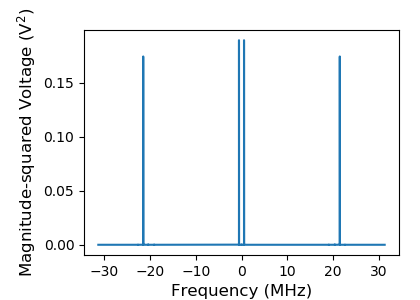
\includegraphics[width=.8\linewidth]{7-1/l_power}
	\caption{Lower sideband $\nu_{RF} = \nu_{LO} - \Delta \nu$.}
	\label{fig:low_pow}
\end{minipage}%
\begin{minipage}{.5\textwidth}
	\centering
	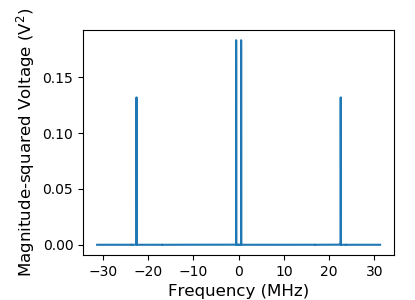
\includegraphics[width=.8\linewidth]{7-1/h_power}
	\caption{Upper sideband $\nu_{RF} = \nu_{LO} + \Delta \nu$.}
	\label{fig:high_pow}
\end{minipage}
\end{figure}

Following the trigonometric manipulations introduced in the discussion of our methods, we may observe that the differences between the power spectra for the lower (figure \ref{fig:low_pow}) and upper (\ref{fig:high_pow}) lie in the $\cos(2\nu_{LO} \pm \Delta \nu$) term. That is to say, we find the power spikes for the difference-signal at the same location in both spectra, and the sum-signal at slightly different locations: gap of 1 MHz between the two pairs, as we would expect.

We demonstrate the results of a Fourier filter in figure \ref{fig:filtered}. When we take the Fourier transform of the sampled signal (\ref{fig:low_display}) and zero out the sum components, we can take the inverse Fourier transform and extract the difference sine wave. The waveform is not slightly corrupted by noise; in the interest of rigor we have not zeroed out anything but the sum spikes.

\begin{figure}
\centering
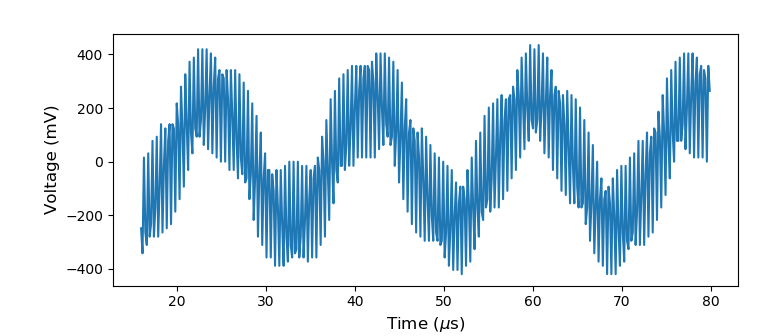
\includegraphics[width=.8\linewidth]{7-1/low_osc}
\caption{Waveform in the case where $\nu_s = 62.5$ MHz and where $\nu_{RF} = \nu{LO} - \Delta \nu = 10.45$ MHz. The largest-frequency signal is that of the sum, $2 \nu_{LO} + \Delta \nu$ = 23.1 MHz.}
\label{fig:low_display}
\end{figure}

\begin{figure}
\centering
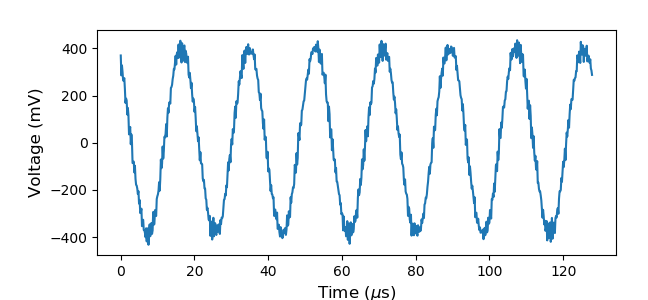
\includegraphics[width=.8\linewidth]{7-1/filtered}
\caption{}
\label{fig:filtered}
\end{figure}

% subsection{7.2}

\begin{figure}
\centering
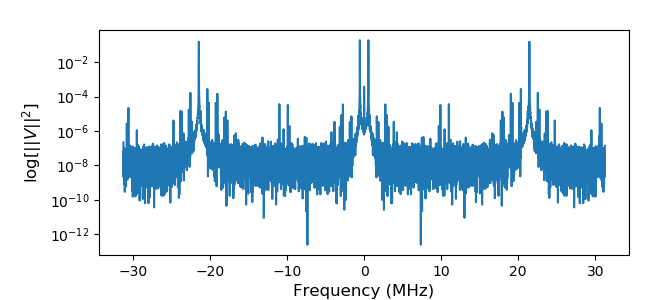
\includegraphics[width=.8\linewidth]{7-2}
\caption{}
\label{fig:intermods}
\end{figure}

The mixers are non-ideal but instead perform $approximate$ multiplication with nonlinear diodes. In figure \ref{fig:intermods}, we demonstrate a repetition of pairs of lines symmetric about the zero frequency. We can see harmonics of the difference signal as pairs of spikes that fall off steeply, fading into noise at about $\pm$ 4 MHz. Incidentally, the spikes close to $\pm$ 10 MHz appear not to be harmonics but rather the original signals re-emerging.

To control our investigation of the single-sideband (SSB) mixer, we first wired components as described in the methods section, but then used an approximately 5 cm cable to connect the RF inputs (approximating zero delay). %Figures \ref{fig:pln} and \ref{fig:phn} show the power spectra obtained with this setup. 

\begin{figure}
\centering
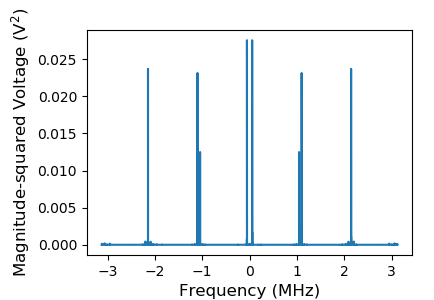
\includegraphics[width=.8\linewidth]{7-3/pln}
\caption{SSB with $\approx$ zero delay. $\nu_{LO} = \nu_s - \Delta \nu$. The boundaries reveal that the sampling frequency was only 6.25 MHz.}
\label{fig:failure}
\end{figure}

\section{Conclusions}

% ?? You probably want to put the following in the conclusion

\quad \quad Phase is defined with respect to some reference point; although we can discuss the phase of a single sample through its voltage spectrum, phase only becomes physically meaningful when we have multiple signals to compare. Therefore, we would find voltage spectra to be physically insightful when we are investigating multiple signals at once. Power spectra are useful for both single and simultaneous signals but, as we have seen, combined signals lead to results about the combination, and information about the individual constituents is less accessible. However, power spectra immediately provide explicit characteristics of signals, so their utility in examining individual signals is demonstrated.

We qualitatively demonstrated the Nyquist criterion by sampling signals at various fractions of the sampling frequency, and examining power spectra. We showed the manifestations of the divergence between the ideal continuous Fourier transform and the real-world discrete Fourier transform by changing the size of the frequency intervals and discussing its impacts on leakage power and frequency resolution.

We proved our noise data to be Gaussian and demonstrated the effectiveness of averaging signals to decrease noise, with a vaguely predicted power law of $N^{1/10}$ for the proportionality between the signal-to-noise ratio and the number $N$ of data blocks averaged.

We proved our double sideband mixer to work mostly as intended; we showed how the sum and difference signals in the power spectra correspond to the predictions of trigonometric identities. We also showed that we could recover the difference signal via Fourier filtering. However, we also addressed the imperfections of the mixer by showcasing the undesired intermodulation products.

We were unable to provide much experimental demonstration of the correlation and convolution theorems for inconclusive reasons. We were also unable to offer data on the single-sideband mixer due to data collection blunder.

\section{Acknowledgments}

I collected and re-collected data for lab activities 5.2-5.7, as well as data for section 7.1. Mehdi Arhor provided example analyses for sections 5.6-5.7 and section 7 activities. Rebecca Gore typed up methods and documented the specific values and amplitudes that we should use when collecting data.

Theory and background provided by Aaron Parsons. "LAB 1: Exploring Digital Sampling, Fourier Filtering, and Heterodyne Mixers." 2020.

\end{document}